\chapter[Introduction]{Introduction}{Introduction}
\label{chap:intro}
{\Huge \calligra T}his thesis focuses 

\section{Motivation}
Motivate ...

\section{Background}
Tell the background. Cite reference \cite{samanta2020direct} and \cite{samanta2018fast}. You can add an image here as shown in Fig. \ref{figure:labelName}. You can add table as shown in Table \ref{Table:labelOfTable}

\begin{table}[h]
	\renewcommand{\arraystretch}{1.3}
	\caption{Caption of table} \label{Table:labelOfTable} \centering
	\begin{tabular}{l|l|l}
		\hline \hline
		Heading 1           & \multicolumn{2}{c}{Heading 2}   \\ \hline
		& Sub Heading 1 & Sub Heading 2     \\ \hline
		Item 1      & 123 \%       & 456 \\
		Item 1      & 123 \%       & 456 \\
		\hline
	\end{tabular}
\end{table}

\begin{figure}[h] 
	\centering
	{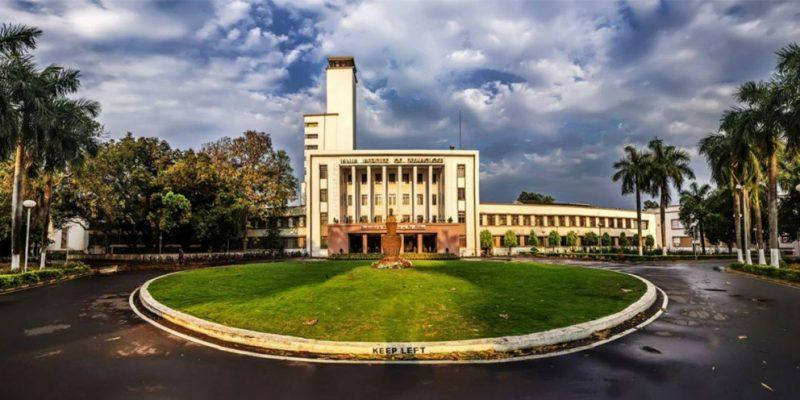
\includegraphics[width=120mm]{Chapter_intro/figs/img1}}
	\caption{Caption of Figure} \label{figure:labelName}
\end{figure}

\section{Research Issues}
List the issues here.

\section{Research Objectives}

This thesis objectives can be listed as follows:

\begin{itemize}
	\item obj1
	\item obj2
	\item obj3
\end{itemize}

\section{Contributions}
The main contributions of this thesis can be summarized as follows:
\begin{itemize}
	\item \textbf{Developed XYZ:} Say something here.
	\item \textbf{Creation of PQR:} Text here.
\end{itemize}

\section{Thesis Organization}

\section{Conclusions}
Summary of the chapter goes here